\subsection{Plane Extraction}

To perform the plane extraction, we used the region growing algorithm described in the lectures in the context of system 6. In general, we concentrated on tailoring the algorithm so that it worked quickly and effectively, rather than re-implementing functionality that was already present in the example code. Our main innovation was to use our knowledge of the problem to optimize the process of patch selection. Aside from that change, and the pre-processing described in the previous section, our main modifications to the example code consisted of tuning parameters of the region growing algorithm so that it worked well with the supplied data. We describe both the patch selection and region growing here. The matlab code to perform the plane extraction is shown in section \ref{PlaneExtractionCode} of this report.

\subsubsection{Patch Selection}

The approach that the example code takes to patch selection can be summarized by the following three step algorithm (implemented in the function \emph{select\_patch.m} in the example code:

\begin{enumerate}
	\item Pick a seed point at random from the point cloud
	\item Create a patch around that point by looping through each point and selecting the points whose euclidean distance from the seed point is below a certain threshold. If less than a certain number of points have been added to the patch when this process is complete, return to step 1
	\item Fit a plane to the patch using the least squares approach implemented in \emph{fitplane.m} in the example code. If the residual least squares fitting error is higher than a certain threshold, throw out the current patch and return to step 1 (as the patch probably includes points from more than one plane
\end{enumerate}

An approach such as this one, which relies on seed points are chosen at random, has a number of drawbacks in the context of the current problem. Two major drawbacks are the following:

\begin{enumerate}
	\item \emph{It is slow.} The seed points may be on or close to edges, or in places where not enough neighbors exist to form a plane, quite often, meaning that the algorithm has to loop through all of the data points multiple times before an appropriate patch is found. For an image with a large number of pixels, this takes a long time.
	\item \emph{It does not distinguish between planes.} The seed points may lie on any plane in the image, so the while the set of planes returned by the algorithm might contain the correct planes, the set is not ordered. As a result, it is necessary to perform the additional step of matching the planes to each other in the different images after the plane extraction has taken place
\end{enumerate}

To overcome these drawbacks, we used a different approach, using our knowledge of the problem to approximate the position of appropriate seed points for the initial patches on each of the three planes. To do that we extracted the closest point in terms of Z in the range data, which was the corner of the cabinet, and then extracted three seed points with the following equations:

\begin{equation*}
	\begin{split}
	\text{rightPoint } &= (\text{cornerPoint(x)} + 40, \text{ cornerPoint(y)} - 20, \text{ cornerPoint(z)} + 30) \\
	\text{leftPoint } &= (\text{cornerPoint(x)} - 40, \text{ cornerPoint(y)} - 20, \text{ cornerPoint(z)} + 30) \\
	\text{topPoint } &= (\text{cornerPoint(x)}, \text{ cornerPoint(y)} + 20, \text{ cornerPoint(z)} + 20) \\
	\end{split}
\end{equation*}

Here the rightPoint is our approximation for the seed point for the initial patch for the right side of the cabinet, leftPoint for the left side, and topPoint for the top half (see Figure \ref{fig:points}). By using these approximation points we found three seed points in the point cloud that were closest to the approximations, and each of them respectively turned out to be on the planes we wanted to extract. This meant that we could use them as out initial patches for region growing on each plane and not have to randomly select seed points for our initial patches. The patches we acquired using these points were computed using a distance tolerance of 5.

\begin{figure}[H]
	\centering
	\begin{subfigure}[b]{0.45\textwidth}
		\centering
		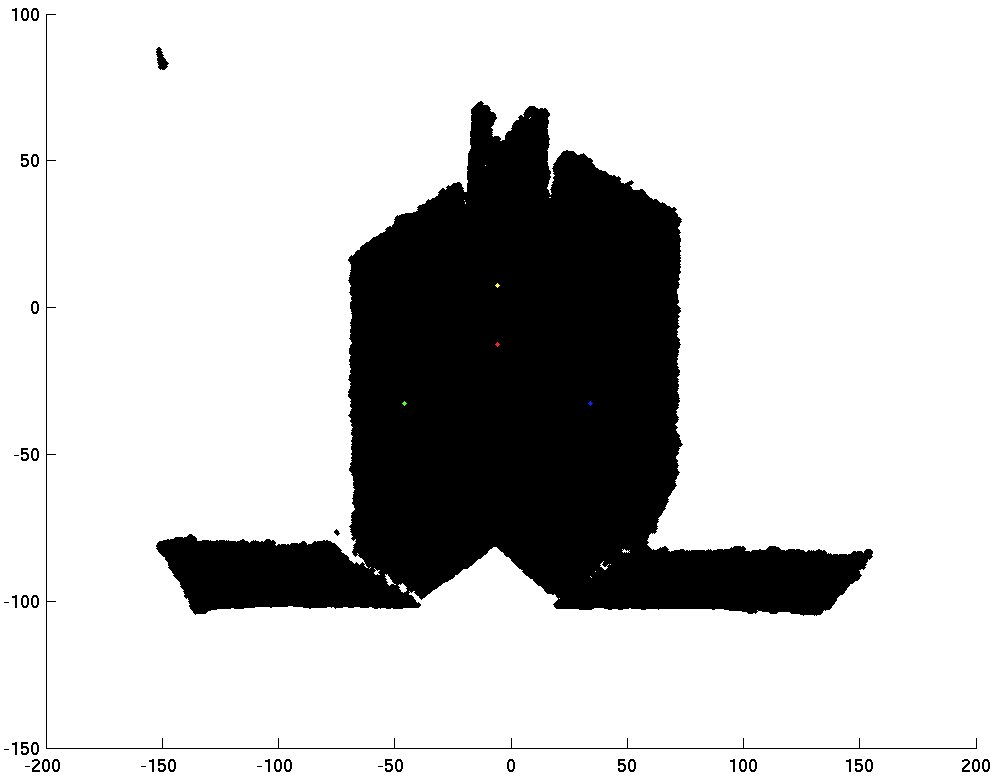
\includegraphics[width=\textwidth]{Images/4-Points(1).png}
		\caption{}
		\label{fig:points}
	\end{subfigure}%
	\hspace{1cm}
	\begin{subfigure}[b]{0.45\textwidth}
		\centering
		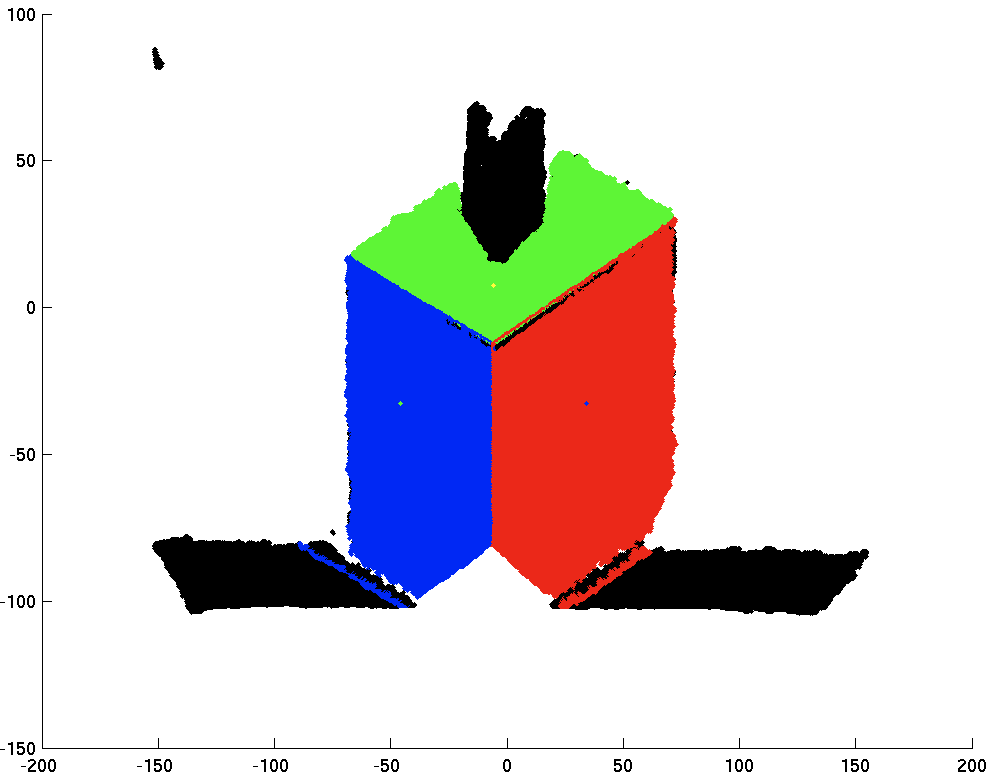
\includegraphics[width=\textwidth]{Images/5-RegionGrowing(1).png}
		\caption{}
		\label{fig:regionGrowing}
	\end{subfigure}
	\caption{Reduced point cloud data with the corner point (red) and the three approximation points for the three planes (a) and region growing with initialization on the closest patch to the points (b).}
\end{figure}

\subsubsection{Region Growing}

To perform the region growing itself, we used the example code from system 6 in the lectures, with the following settings for the relevant parameters:

\begin{itemize}
	\item In \emph{getallpoints.m}, we used a plane tolerance of 1 and point distance tolerance of 150. By having a low plane tolerance we acquired more accurate regions and with such a large point distance tolerance the growing only needed about 5 iterations
	\item In the main region growing loop, we specified that when the number of new points in a region exceeded the number of points already in the region plus 50 then a plane is (re)fitted to the region. The region growing stops when the least square fitting error of that plane is bigger than 30\% of the number of new points.
\end{itemize}
